Wie im vorigen Abschnitt beschrieben wurde, fehlt der bisherigen Beschreibung von Webservices der semantische Aspekt. Unter \emph{semantischen \acl{WS}} versteht man solche \acl{WS}, deren Beschreibung neben der konkreten technischen Aspekten zur Anbindung auch Information zur abgebildeten "`Welt"' enthalten. In diesem Abschnitt erläutere ich deren Grundlagen.

\subsection{Semantik}

Die \emph{Semantik} (griechisch, "`Bezeichnung"') beschreibt das Wesen von Dingen und ermöglicht die Interpretation und Übertragung von Konzepten auf konkrete Begebenheiten. Semantik ist die Grundlage jeglicher Kommunikation und umgibt uns überall. Bereits in jungen Jahren lernen wir, dass ein über einem Weg hängender Kasten, aus dem uns ein Licht rot anstrahlt eine \emph{bestimmte} Bedeutung hat. Nach einiger Zeit verbinden wir damit intuitiv: "`Halt, hier geht es nicht weiter."' Wichtig ist allerdings, dass die scheinbar eindeutige Verbindung zwischen der Farbe "`Rot"' und dem Konzept "`Nicht weiter gehen!"' kontextabhängig ist. Begegnet uns ein leuchtendes Rot auf einem Apfel, wissen wir, dass das Obst frisch und genießbar ist. Die Bedeutung "`Halt!"' der Farbe Rot verdreht sich in diesem Kontext in das Gegenteil: "`Iss mich!"'.

Wie schon auf Seite \pageref{l:intro-loosecoupling} beschrieben, ist Voraussetzung für eine Service-Infrastruktur mit loser Kopplung, dass die Bedeutung der Aufgabe, die mit dem Webservice abgebildet wird automatisch ermittelt werden kann.

Beschreibt man einen Webservice z.B. mittels der \ac{WSDL}, legt man damit lediglich den Syntax für die vom Webservice verarbeiteten Anfragen fest. Die Bedeutung der Funktionalität und der übertragenen Daten erschließt sich daraus nicht. Sie entsteht lediglich in der Interpretation der Benutzer des Dienstes. 

In Listing \ref{code:wsdl} auf Seite \pageref{code:wsdl} findet sich eine \ac{WSDL} für der Webservice "`PeopleAsk"'\footnote{http://peopleask.ooz.ie/}, mit dem sich die aktuell in Google gestellten Fragen abrufen lassen. Beschrieben werden die Entitäten \emph{GetQuestionsAbout} mit dem Attribut \emph{query} und \emph{GetQuestionsAboutResponse}, das eine Liste mit Strings ist. Aus dem Dokument geht jedoch nicht hervor, dass eigentlich \emph{Suchanfragen} einer \emph{Suchmaschine} zurückgegeben werden --- dieses Wissen entsteht aus Informationen, die nur außerhalb der Schnittstellenbeschreibung zugänglich sind.

Es fehlt also eine Komponente, die dem reinen Akt der Datenübertragung ein inhaltlichen Beschreibung, hinzufügt und das zudem noch in maschinenlesbarer Form. In der Informatik sind das \emph{Ontologien}.

Ontologien sind die \emph{Spezifikation eines Konzepts}. \emph{Spezifikation} bedeutet dabei eine formale und deklarative Repräsentation, die damit automatisch maschinenlesbar ist und Missverständnisse ausschließt. Ein \emph{Konzept} ist die abstrakte und vereinfachte Sicht der für das Konzept relevanten Umgebung. Ontologien beschreiben aus der Sicht des Dienstanbieters die Zusammenhänge in der Umgebung, auf die durch den Webservice implizit zugegriffen wird. In \cite[S.31]{dcswe} liefert Devedžić zum bessern Verständnis dieses Bildnis: Möchte eine Person über Dinge aus der Domäne \emph{D} mit der Sprache \emph{L} sprechen, beschreiben Ontologien die Dinge, von denen angenommen wird, dass sie in \emph{D} als Konzepte, Beziehungen und Eigenschaften von \emph{L} existieren.

\subsection{Semantische Beschreibung von \acl{WS}}\label{l:sawsdl}

Mit den \ac{SAWSDL} hat das \ac{W3C} im Jahr 2007 den Entwurf eines Standard vorgelegt, der es ermöglicht Informationen zu diesen Ontologien maschinenlesbar, als Teil einer \ac{WSDL}-Datei, auszuliefern. 

\ac{SAWSDL} ist dabei unabhängig von einem semantischen Konzept und liefert nur den Rahmen um andere semantische Frameworks in \ac{WSDL} zu integrieren --- es wird lediglich vorausgesetzt, dass diese Konzepte anhand von URIs identifierziert werden können \cite[S.61]{ky-sawsdl}. Eine Mögliche Technik zur semantischen Beschreibung bietet die \ac{OWL}, die auf dem \ac{RDF} basiert. In \ac{RDF} werden dabei die Entitäten (in \ac{RDF} "`Ressourcen"' genannt) mit ihren Attributen und Beziehungen untereinander syntaktisch beschrieben. In \ac{RDF} fehlt aber die Möglichkeit, die Beziehungen von Eigenschaften zu beschreiben. Zum Beispiel besitzt ein Buch das Attribut \emph{Autor}. Dass damit aber eine weitere Ressource gemeint ist (eine \emph{Person} mit der Rolle \emph{Autor}) lässt sich in einem \ac{RDF}-Dokument nicht hinterlegen. Mit der \ac{RDFS} wurde deswegen die Möglichkeit geschaffen, Gruppen zusammengehöriger Ressourcen und ihrer Beziehung untereinander zu beschreiben. Mit \ac{OWL} ist es schließlich möglich, Ontologien in Form von Klassen, Eigenschaften, Instanzen und Operationen zu beschreiben.Abbildung \ref{f:ewsss} liefert einen Überblick über den Zusammenhang der vorgestellten Technologien.

\begin{figure}[ht]
\centering
\parbox{0.85\textwidth}{
    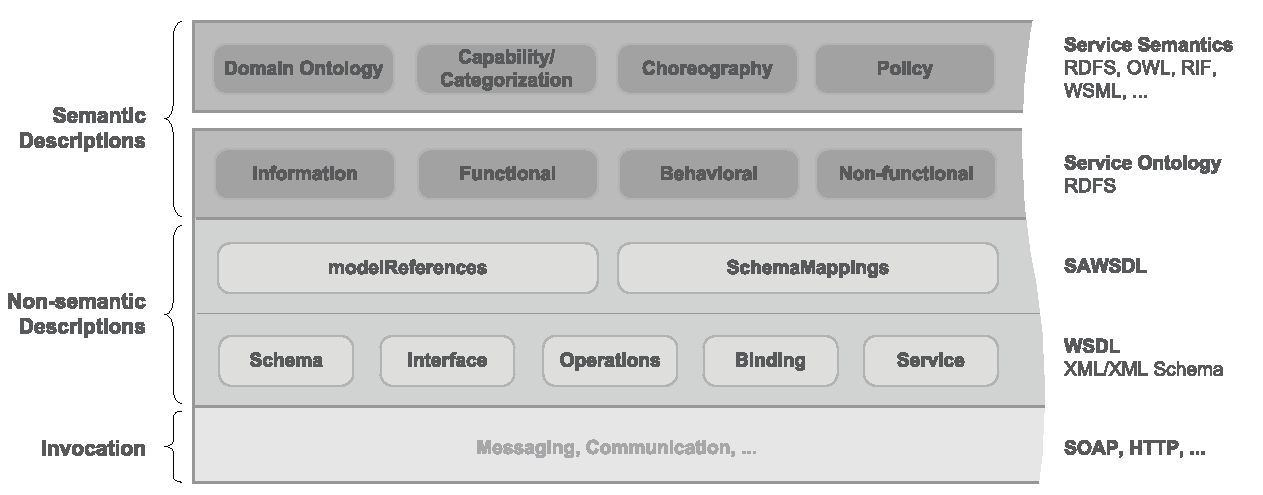
\includegraphics[width=0.85\textwidth]{media/Extended-Web-Service-Specification-Stack.pdf}
    \caption{\emph{Extended Web service specification stack} \cite[S.63]{ky-sawsdl}. Die Hauptbeschreibungssprache \ac{WSDL} ist eng an die darunterliegenden Kommunikationsprotokolle gekoppelt. \ac{SAWSDL} verbindet als Schicht darüber \ac{WSDL} mit den übergeordneten semantischen Informationen, wobei die Service-Ontologien die allgemeinen Aspekte von \acl{WS} beschreiben und die Service-Semantik die domainspezifischen Aspekte formuliert.}
    \label{f:ewsss}
}
\end{figure}

In \ac{WSDL} werden \acl{WS} auf einer syntaktischen Ebene beschrieben. Es wird festgelegt, wie die auszutauschenden Nachrichten \emph{aussehen} und an welchen Endpunkten der \ac{API} diese zum Einsatz kommen, nicht jedoch was sie \emph{bedeuten}. In \ac{WSDL} werden die abstrakten Elemente \emph{Element Declaration}, \emph{Type Definition} und \emph{Interface} verwendet, um einen Webservice allgemein zu beschreiben. In diesen Elementen spielen die technischen Einzelheiten, wie z.B. das verwendete Protokoll, keine Rolle. Ein \emph{Type} entspricht dabei einem Objekt aus der Domäne, ein \emph{Element} beschreibt ein Attribut dieses Objekts. Ein \emph{Interface} beschreibt die Operationen und deren Parameter, die von der Schnittstelle unterstützt werden. In Listing \ref{code:wsdl2} auf Seite \pageref{code:wsdl2} findet sich ein einfaches Beispiel einer \ac{WSDL}-Datei. Abbildung~\ref{f:wsdlmodel}\footnote{Quelle: http://www.w3.org/TR/wsdl20-primer/}, die das Datenmodell \ac{WSDL}-Datei zeigt, liefert einen Überblick über die Elemente in \ac{WSDL}.

\begin{figure}[ht]
\centering
\parbox{0.85\textwidth}{
    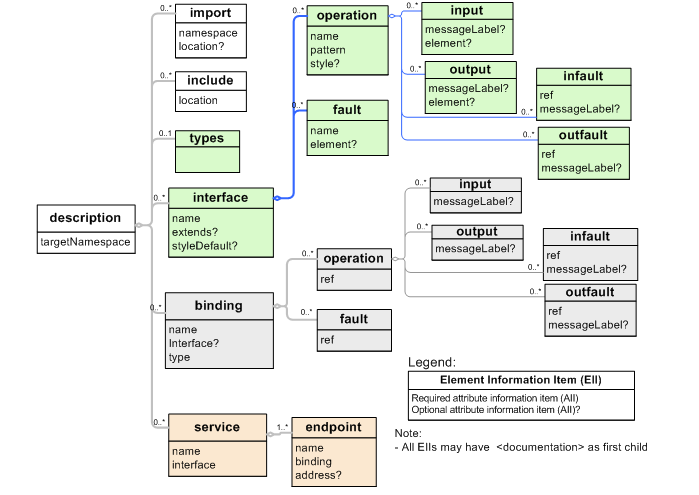
\includegraphics[width=0.85\textwidth]{media/WSDL20InfosetModel.png}
    \caption{Das Datenmodel von \ac{WSDL}}
    \label{f:wsdlmodel}
}
\end{figure}

\ac{SAWSDL} führt nun für diese drei Elemente zusätzlich Attribute ein, um deren semantische Bedeutung zu beschreiben \cite[S.62ff]{ky-sawsdl}:

\begin{itemize}
\item \texttt{modelReference} definiert eine Beziehung zwischen einem der definierten Komponente in der \ac{WSDL} und einem Objekt im semantischen Modell. Diese Attribut kann auf jedes \ac{WSDL}- oder XML-Schema-Element angewendet werden. Der Wert des Attributes ist dabei eine oder mehrere URIs, die auf ein semantisches Modell verweisen.
\item Die Attribute \texttt{liftingSchemaMapping} und \texttt{loweringSchemaMapping}, die auf Typedefinitionen definiert werden können, spezifizieren das Mapping zwischen semantischen Daten (z.B. \ac{RDF} und XML) sowie umgekehrt. Hierbei ist es auch möglich, mehrere Mappings je Typ zu definieren, um verschiedene Repräsentation je Kontext zu ermöglichen. Die \emph{lifting}- und \emph{lowering}-Transformationen sind nützlich, wenn von einem semantischen Client aus mit einem \acl{WS} kommunziert wird. Für eine Anfrage werden dann die semantischen Daten in das Anfrage-Format des Client durch \emph{lowering} transformiert, die Antwort wird dann durch \emph{lifting} wieder in ein semantisches Format konvertiert. Dieses Verfahren kommt auch bei der Verwendung einer gemeinsamen Ontologie zum Einsatz --- ein automatischer Vermittler kann dabei die Daten zwischen zwei Endpunkten mit den \emph{Lifting}-Informationen des Anfragers und den \emph{Lowering}-Informationen des Empfängers vermitteln. Sprachen für das \texttt{liftingSchemaMapping} sind z.B. \emph{XSLT} oder \emph{XQuery}, für das \texttt{loweringSchemaMapping} \emph{SPARQL} (eine Abfrage-Sprache für \ac{RDF}) gefolgt von \emph{XSLT} oder \emph{XQuery}.
\end{itemize}

Abbildung \ref{f:sawsdl} liefert eine Übersicht über die Integrationspunkte von \ac{SAWSDL} in \ac{WSDL}.

\begin{figure}[ht]
\centering
\parbox{0.85\textwidth}{
    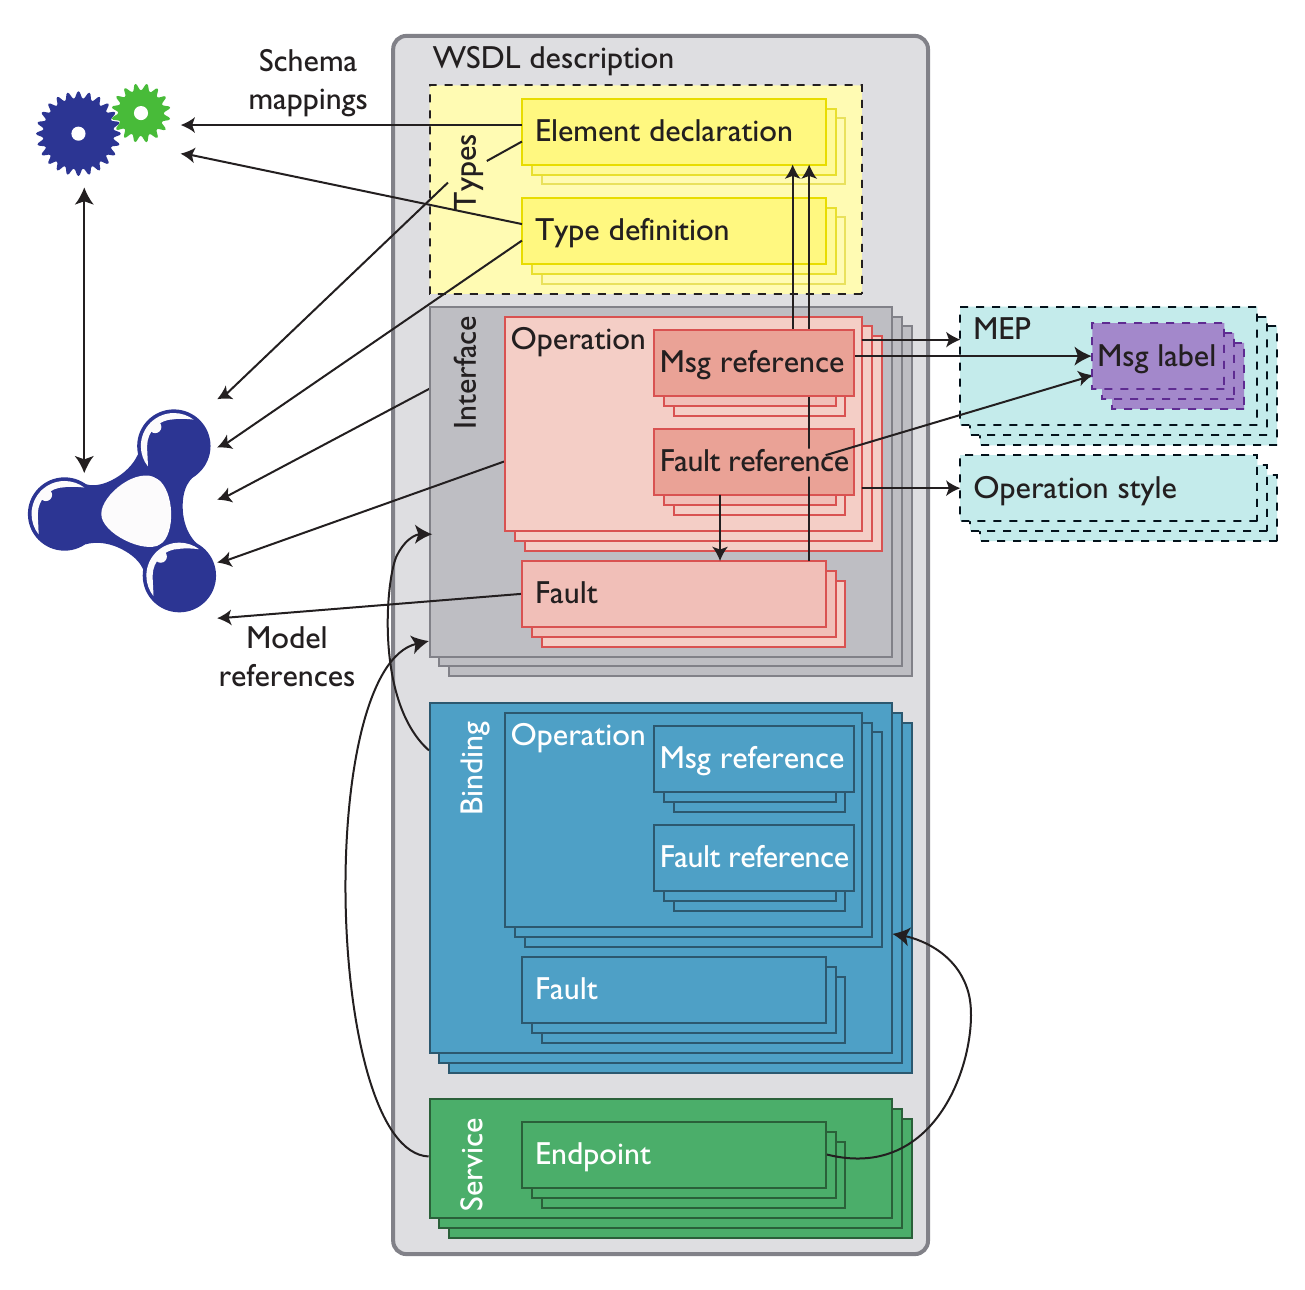
\includegraphics[width=0.85\textwidth]{media/sawsdl.png}
    \caption{\ac{WSDL} mit \ac{SAWSDL}. Diese Abbildung zeigt die \ac{WSDL}-Kompüonenten und die zugehörigen \ac{SAWSDL}-Erweiterungen, die zu Konzepten zu semantischen Spezifikation der Domain oder zum Data-Mapping verweisen. \cite[S.61]{ky-sawsdl}
}
    \label{f:sawsdl}
}
\end{figure}

\subsection{\ac{SAWSDL} verwenden}

Der Standardisierungsprozess des \ac{W3C} fordert von allen Entwürfen für neue Standards, dass diese auf ihrer vollständige Implementierbarkeit überprüft werden müssen, bevor sie letztendlich zur Empfehlung erhoben werden dürfen. Jedes Feature der Spezifikation muss funktional in mindestens einer Implementierung vorliegen und idealerweise zwischen zwei Implementierungen interoperabel sein. Damit eine Arbeitsgruppe, also diejenigen die neue Standards entwickeln, zu einer Empfehlung kommen kann, muss diese Gruppe einen Implementierungsreport vorlegen. Im Bericht der \ac{SAWSDL}-Arbeitsgruppe\footnote{http://www.w3.org/2002/ws/sawsdl/CR/} finden sich Implementierungen in mehreren Bereichen des Standards.

Direkte Implementierungen von \ac{SAWSDL} sind Parser-\ac{API}s, die die Erweiterungen anderen Anwendungen und Werkzeugen zur Verfügung stellen, mit denen \ac{WSDL}-Dokumente semantisch beschrieben werden können. So wurde die \emph{Woden API für WSDL 2.0}\footnote{http://ws.apache.org/woden/} und die \emph{WSDL4J API für WSDL
1.1}\footnote{http://sourceforge.net/projects/wsdl4j/} so erweiterte, dass diese \ac{SAWSDL}-Informationen auslesen können. Auf diesen Bibliotheken bauen viele Jaba-basierte Werkzeuge auf, wie z.B. der Apache Webservice Stack \emph{Axis 2}\footnote{http://axis.apache.org/axis2/java/core/}. Auch zwei GUI-Werkzeuge, mit denen \ac{WSDL}-Dokumente semantisch beschrieben werden können, unterstützen den Standard: \emph{Radiant}\footnote{http://lsdis.cs.uga.edu/projects/meteor-s/downloads/index.php?page=1} von der \emph{University of Georgia} und das \acl{WSMO} \emph{Studio}\footnote{http://www.wsmostudio.org/} von \emph{Ontotext}. Da \ac{SAWSDL} wie beschrieben eine Spezifikation zum Hinzufügen von Semantiken ist, liegt sein Wert vor allem in den Anwendungen, die von diesen Semantiken gebrauch machen. Im Implementierungsreport werden mehrere solche Anwendungen erwähnt.
Insbesonderes kann man \ac{OWL-S} und \ac{WSMO}, die zu den gängigsten Frameworks für semantische Webservices zählen,  mit \ac{SAWSDL} in \ac{WSDL}-Dokumente integrieren. Mit \emph{Lumina}\footnote{http://lsdis.cs.uga.edu/projects/meteor-s/downloads/Lumina/} von der \emph{University of Georgia} können mit \ac{SAWSDL} beschriebene \acl{WS} "`entdeckt"' werden und die \emph{Semantic Tools for Web Services}\footnote{http://lists.w3.org/Archives/Public/public-ws-semann/2006Oct/0030.html} von IBM sind in der Lage, semantische Daten zu verknüpfen und vermitteln.
In \ac{SAWSDL} ist es sogar möglich, semantische Beschreibungen für die \emph{Business Process Execution Language for Web Services}\footnote{http://www.ibm.com/developerworks/library/specification/ws-bpel/} (BPEL4WS) zu hinterlegen, ein Anwendungsfall der ursprünglich nicht von der Arbeitsgruppe berücksichtigt wurde. \cite[S.63]{ky-sawsdl}

Auch für die \emph{Eclipse IDE} gibt es mit \emph{Jena}\footnote{http://jena.sourceforge.net/} ein Plug-In dass bei der Entwicklung von semantischen Webservices in Java unterstützt.

Wie in diesem Abschnitt gezeigt wurde, sind also die theoretischen Grundlagen und praktischen Hilfsmittel zur semantischen Beschreibung von \acl{WS} vorhanden.

% MARK

\subsection{\ac{SAWSDL} und \ac{REST}?}

Auch wenn dass \ac{W3C} in seinen Standards und Entwürfen keine Vorgaben zur eigentlichen Realisierung der Kommunikation mit \acl{WS} macht, ...

A Web service is a software system designed to support interoperable machine-to-machine interaction over a network. It has an interface described in a machine-processable format (specifically WSDL [Web Services Description
Language]). Other systems interact with the Web service in a manner prescribed by its description using SOAP-messages, typically conveyed using
HTTP with an XML serialization in conjunction with other Web-related standards.


Mit \ac{REST} hat sich gerade im Bereich webbasierter Schnittstellen ein Zugriffsprotokoll 

\begin{itemize}
\item \cite{ma-sawslrest}
\item \cite{xn-sss}
\end{itemize}